\documentclass{beamer}
\usetheme{Luebeck}

\usepackage{animate}

\title{Interfacing a VGA monitor with an FPGA}
\subtitle{P\&S Course iCEBreaker FPGA for IoT Sensing Systems}
\institute{ETH Zürich}
\author{Stefan Gloor}
\date{December 22, 2021}

\begin{document}

\begin{frame}
	\titlepage
\end{frame}

\begin{frame}{Goal of the project}
	\begin{itemize}
		\item Implementation of the VGA protocol
		\item Ability to display arbitrary images in color
		\item Interactive animation for demo (e.g. game)
	\end{itemize}
\end{frame}

\begin{frame}{Necessary hardware}
	\begin{minipage}{0.49\textwidth}
		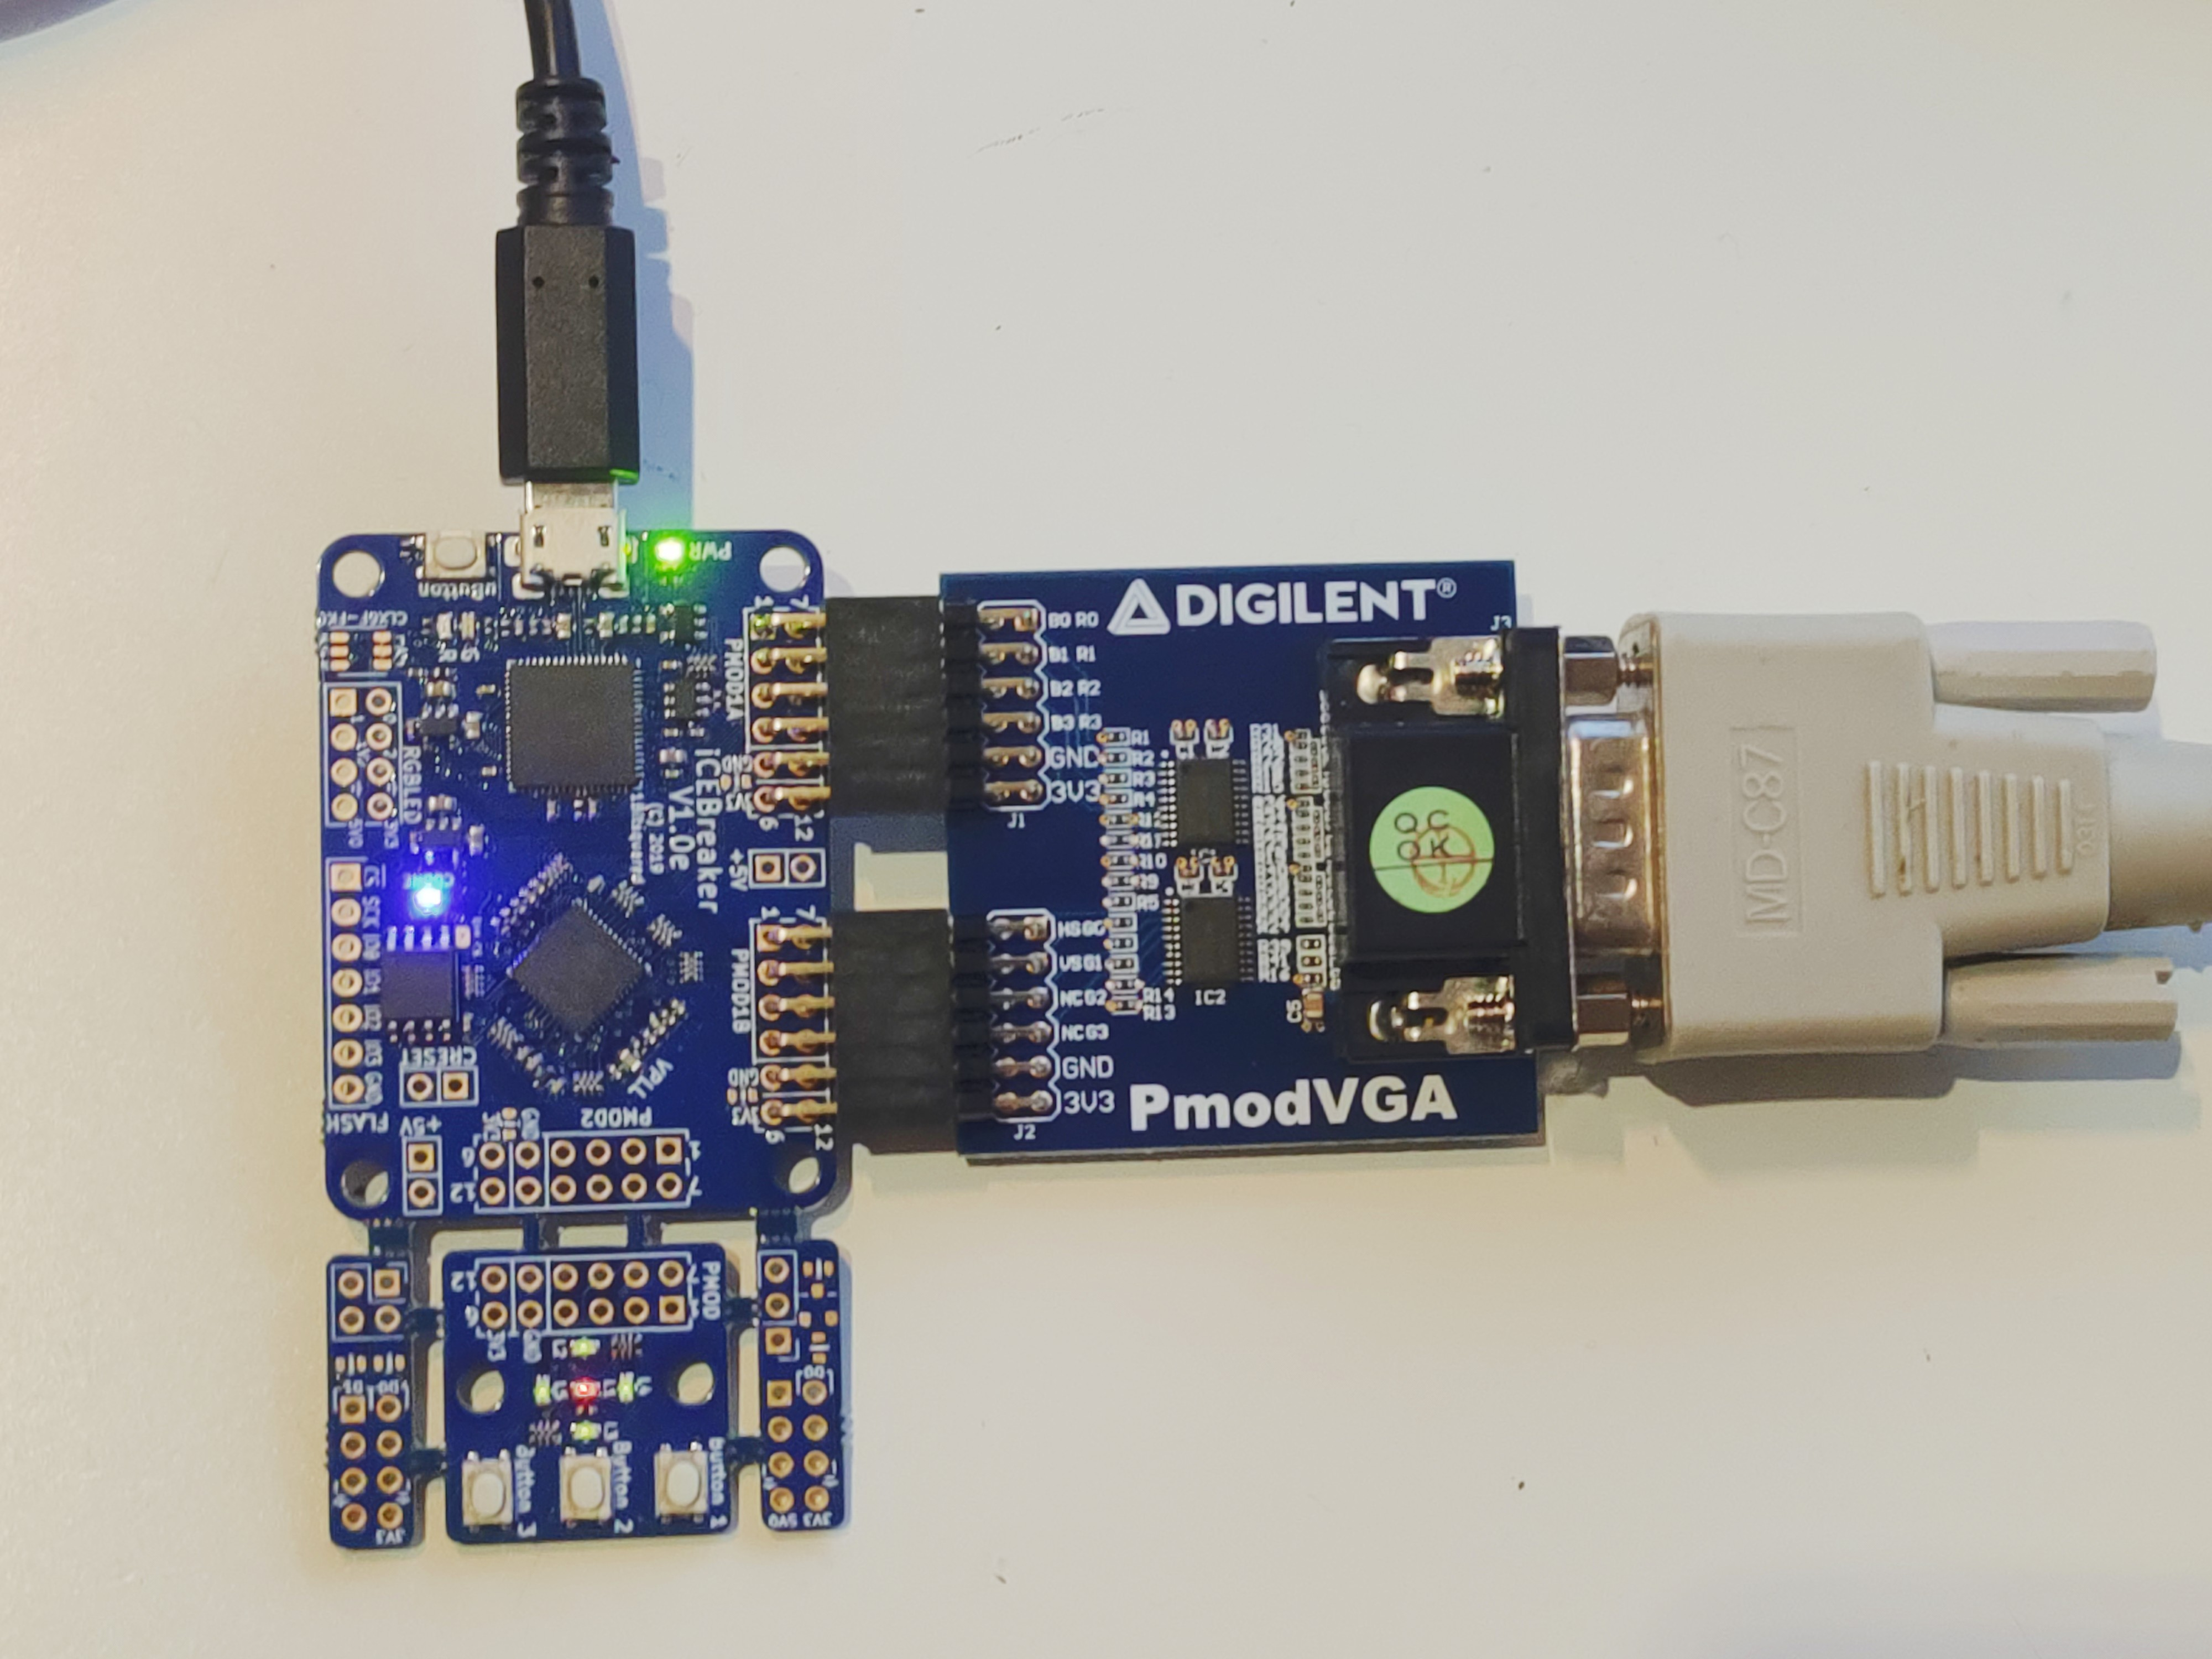
\includegraphics[width=\textwidth]{../hardware.jpg}
	\end{minipage}
	\begin{minipage}{0.49\textwidth}
		\begin{itemize}
			\item iCEBreaker FPGA Board
			\item VGA Pmod
			\item Standard VGA cable and monitor
		\end{itemize}
	\end{minipage}
\end{frame}

\begin{frame}{VGA interface}
	\begin{itemize}
		\item The VGA protocol uses purely analog RGB signals.\\
		$\implies$ this means we need to convert digital 
		to analog signals.
	\item Pixel data is transmitted by ``scanning" 
		across the screen.
	\item Frame and line synchronisation is done 
		by digital sync signals on dedicated lines.
	\end{itemize}
	\begin{figure}
	\begin{tabular}{l|l|l}
		\textbf{Pin \#} & \textbf{Signal} & \textbf{Description}\\
		1			& R & Analog red color\\
		2			& G	& Analog green color\\
		3			& B & Analog blue color\\
		13		& HSYNC & Horizontal synchronisation (line)\\
		14		& VSYNC & Vertical synchronisation (frame)
	\end{tabular}
	\caption{Most essential VGA pins}
\end{figure}
\end{frame}

\begin{frame}{VGA interface}
	\begin{minipage}{0.66\textwidth}
	
\includegraphics[width=\textwidth]{../figures/signals-figure0.pdf}
	\end{minipage}
	\begin{minipage}{0.32\textwidth}
		\begin{itemize}
			\item Pixel frequency of 25.175 MHz
			\item Horizontal and vertical pixel counters
			\item Create sync pulses depending on counters
		\end{itemize}
	\end{minipage}
\end{frame}

\begin{frame}{Pmod VGA}
	\begin{minipage}{0.66\textwidth}
		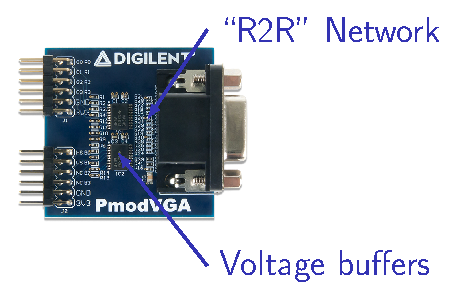
\includegraphics[width=\textwidth]{../figures/pmod-figure0.pdf}
	\end{minipage}
	\begin{minipage}{0.32\textwidth}
		\begin{itemize}
			\item Bus transceivers ensure stable voltage 
			\item 4-Bit D/A conversion by simple resistor network
		\end{itemize}
	\end{minipage}
	\footnote{Image based on Digilent reference:
	\url{https://digilent.com/reference/_media/reference/pmod/pmodvga/pmodvga-1.png}}
\end{frame}

\begin{frame}{My Implementation}
	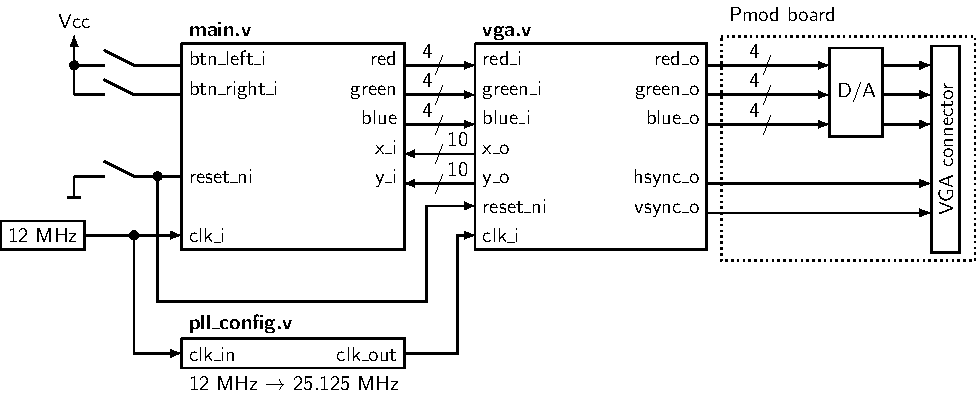
\includegraphics[width=\textwidth]{../figures/diagram-figure0.pdf}
\end{frame}

\begin{frame}{Pong game demo}
\end{frame}

\begin{frame}{Questions?}
	\begin{minipage}{0.49\textwidth}
		\begin{center}
		
\includegraphics[width=\textwidth]{../qr.png}
		The project is on Github!
	\end{center}
	\end{minipage}
	\begin{minipage}{0.49\textwidth}
	Thank you for your attention.
	\end{minipage}
\end{frame}

\end{document}
